% !TeX root = scaffold-70.tex
\renewcommand{\imagepath}{../70-supervised/img}

\chapter{Supervised Analysis: Zero-Shot Classification}\label{ch:supervised}
In this chapter, the newspaper articles \todo{continue}

\section{Analysis Procedure}
In contrast to topic modelling, in the case of zero-shot classification (see section~\ref{ch:zero_shot}) training and optimization has already been performed by the model provider. The employed BART model~\autocite{lewis_bart_2020} \todo{decide for one kind of reference} is not trained on any inputs and is not altered during the classification process. It can assign a relative semantic proximity $p_{i, l}$ to a given newspaper article $i$ for each label $l$ out of a set of labels. This quasi-probability represents how close the meaning of the label is to the meaning of the article. Similar to the procedure in topic modelling, a label was assigned to an article if it had the highest proximity:
\begin{align}
    l_{i} = \max_{l'} p_{i, l'}
\end{align}
Also like in the topic modelling procedure, the information-theoretical entropy \autocite{gray_entropy_2013} for each article was calculated as a measure of how secure the model was of its prediction:
\begin{align}
    H_i = -\sum_{l'} p_{i, l'} \ln p_{i, l'}.
\end{align}
Low entropy signifies that the model could attest a very close proximity of one of the labels, hence an unambiguous assignment of label, whereas a high value of $H_i$ testifies an ambiguous association between the article and the label. As the range of $H$ depends on the number $n_\text{labels}$ of labels, the following normalized variant is used for comparing the model's security across categories:
\begin{align}
    \widetilde{H}_i = \frac{H_i}{\ln n_\text{labels}}
\end{align}

Note that in contrast to the previous chapter's concept of hypertopics, which were human assigned to word lists carrying the articles' semantic information, here the model quantifies the semantic relationship between each article and a given label.

In order to examine the article texts with respect to the aspects motivated in section~\ref{ch:this_thesis}, namely topic, sentiment, success, delinquency, and journalistic style, for each of these aspects one or more categories and a corresponding set of labels was compiled based on the author's intuition and on what would seem interesting for the analysis of role model qualities. The labels used in the analysis are presented in section~\ref{ch:supervised_results} for each category.

\begin{figure}
    \centering
    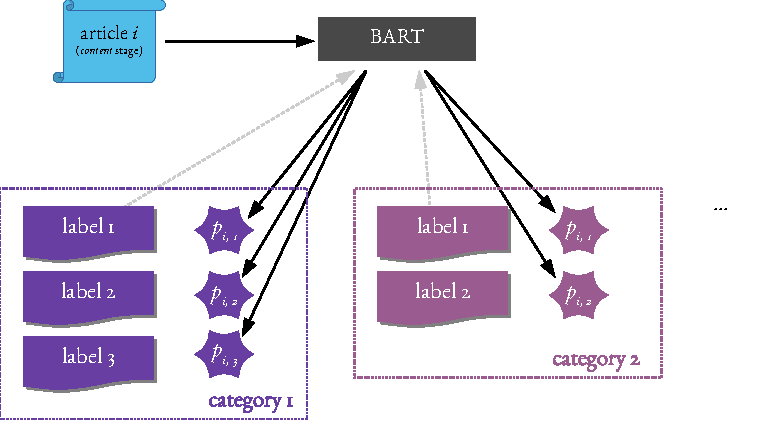
\includegraphics[]{\imagepath/zero_shot_schema.pdf}
    \caption{Schematic of the zero shot classification procedure: An article $i$ is fed into the BART model along with a set of labels, called a category. BART then assigns a relative proximity $p$ to each label for this article. This is repeated for different categories, each having a different set of labels. The BART model itself doesn't depend on any input and is not altered during the whole process.}\label{fig:zero_shot_schema}
\end{figure}

The classification procedure is illustrated in figure~\ref{fig:zero_shot_schema}. The BART model was integrated as suggested in \textcite{huggingfacebart-large-mnli_facebookbart-large-mnli_nodate}. As an input to the model the text in the \textit{content} stage was used, i.e. with most structure of the human language preserved.

\section{Accuracy}\label{ch:supervised_accuracy}
In a first evaluation step, the accuracy of the zero-shot classification was assessed using the human annotated data. To this end, the model made a prediction for each article from the set of labels used in the human annotation process, namely \textit{life}, \textit{movie}, \textit{music}, and \textit{sports}. An accuracy (cf. equation~\eqref{eq:accuracy}) of \SI{57.9}{\percent} was achieved, human annotation and the model-predicted labels are compared in the confusion matrix in figure~\ref{fig:zero_shot_confusion_matrix_topic}, showing that the model especially counts articles that the human annotator marked as sport-related to the label \textit{life}. It was conjectured that this might stem from an alledged semantic proximity of the word ``life'' with ``live sports''. Therefore an alternative set of labels with the \textit{life} label exchanged for \textit{social} was checked. For it an almost equal accuracy of \SI{55.9}{\percent} was achieved, the confusion matrix is shown in figure~\ref{fig:zero_shot_confusion_matrix_topic_l}. Indeed this reduced the confusion with the \textit{label}, however now there was a more pronounced confusion of \textit{social} and \textit{movie}, which is also not surprising considering that reports about movie plots often convey social aspects. Looking at the averaged normalized entropies showed that the model makes more convinced predictions if \textit{life} is replaced by \textit{social}, $\Braket{\widetilde{H}}_\text{life} = 0.87 > 0.77 = \Braket{\widetilde{H}}_\text{social}$.

\begin{figure}
    \centering
    \begin{subfigure}{0.48\textwidth}
        \centering
        \includegraphics[]{\imagepath/zero_shot_confusion_matrix_topic.pdf}
        \caption{topic}\label{fig:zero_shot_confusion_matrix_topic}
    \end{subfigure}
    \hspace{0.03\textwidth}
    \begin{subfigure}{0.48\textwidth}
        \centering
        \includegraphics[]{\imagepath/zero_shot_confusion_matrix_topic_l.pdf}
        \caption{topic (soc.)}\label{fig:zero_shot_confusion_matrix_topic_l}
    \end{subfigure}
    \caption{Comparison of the model prediction and the human annotation for the topic and topic (soc.) categories. An accuracy of \SI{}{\percent} was achieved in predicting the human annotation labels. The most pronounced mistake is that the model classifies ...}\label{fig:zero_shot_confusion_matrices}
\end{figure}

The accuracy of the zero-shot approach is hence less than in the topic modelling approach with a pre-trained model (\SI{76}{\percent}). However, the qualitative accuracy recognizable from the confusion matrices is remarkable given that the has not been trained on the corpus of newspaper articles. Since the articles' topics are not unambiguous and also the human-annotated labels are thus subject to uncertainty, the zero-shot approach is arguably still very promising despite its lower accuracy, especially given that it makes it possible to explore all the non-topic aspects of newspaper articles scrutinized in the following.


\section{Results}\label{ch:supervised_results}
In total, the model assigned labels from twelve categories to each article. As was done in the evaluation of topic modelling, the distribution of the articles across the labels of each category was then compared for the low-\gls{ses} and the high-\gls{ses} groups.

Again, a $\chi^2$ contingency test was used to identify significant differences between the article distributions (cf. equation~\eqref{eq:h0_contingency}):
\begin{align}
    \begin{split}
        H_{0, \text{contingency}}: ~~~ &\text{distributions } p_{s, l} \text{ over labels } l \text{ are indepedent of } s\\
    & \text{i.e. } p_{s, l} = p_s \cdot p_l ~~ \forall l, s
    \end{split}
\end{align}
A set of per-label $\chi^2$ tests were conducted to find significant differences in the amount of articles per label were looked for (cf. equation~\eqref{eq:h0_topic}):
\begin{align}
    \begin{split}
        H_{0, \text{ label }l}: ~~~ &\text{number of articles } n_{s, l} \text{ equals expected number } \tilde n_{s, l} \\
        & \text{i.e. } n_{\text{low}, l} = \tilde n_{\text{low}, l} \text{ and } n_{\text{high}, l} = \tilde n_{\text{high}, l},
    \end{split}
\end{align}
with the number of articles $n_s$ in \gls{ses} group $s$, the number of articles $n_l$ associated with label $l$, the total number $n$ of articles, and the expected number of articles $\tilde n_{s, l} = n_s \cdot \frac{n_l}{n}$ per label $l$ and \gls{ses} $s$ assuming independence from \gls{ses}. \footnote{Note that for higher $n_l$, a certain deviation of $n_{s, t}$ from the expectation $\tilde n_{s, t}$ is \textit{less significant} than for a low $n_l$, as the deviation relative to $n_l$ is smaller. Especially for two-label categories, this can lead to potentially unintuitive outcome that the more prevalent label (high $n_l$) in a distribution has less significance in the per-label test than the less prevalent label (low $n_l$). This can be seen can be seen in the results in table~\ref{tab:zero_shot_result_table}, e.g. for the category \textit{prosociality}.}

All examined categories and their respective labels, the respective distributions of articles across the labels, and the results of the $\chi^2$ tests are listed in table~\ref{tab:zero_shot_result_table}. The following paragraphs present these categories and their labels, and analyze the found distributions.
\begin{table}
    \centering
    \resizebox{0.85\textwidth}{!}{../../../build/thesis/70-supervised/zero_shot_result_table.tex}
    \caption{Results of the zero-shot classification for each category along with $\chi^2$ contingency and per-label tests. Legend: $\Braket{\widetilde{H}}$ is the average of the normalized entropy $\widetilde{H}$, *: $p < \SI{1e-1}{}$, **: $p<\SI{5e-2}{}$, ***: $p<\SI{1e-2}{}$.}\label{tab:zero_shot_result_table}
\end{table}

\paragraph{Topics}
The topic aspect of the newspaper articles was covered by the \textit{topic} and \textit{topic (soc.)} categories, as already mentioned in the previous section. Both show similar differences in the distribution of low- and high-\gls{ses} articles, for \textit{topic (soc.)} it is shown in figure~\ref{fig:zero_shot_distribution_topic_l}. In accordance with the findings in topic modelling, the topics of \textit{music} and \textit{sports} have higher prevalence among the low-\gls{ses} group than the high-\gls{ses}, and in turn the \textit{movie} topic is more prevalent in the high-\gls{ses} group. In contrast to topic modelling, here the \textit{life} or \textit{social} label also exposes a significant difference between the \gls{ses} groups, namely more favoured by the high-\gls{ses} group. All these observations are more pronounced in the \textit{distinct-\gls{ses}} dataset.
\begin{figure}
    \centering
    \begin{subfigure}{0.48\textwidth}
        \centering
        \begin{pgfpicture}
            \pgftext{../../../build/thesis/70-supervised/zero_shot_distribution_topic_l.pgf}
        \end{pgfpicture}
        \caption{\textit{mixed-\gls{ses}}}
    \end{subfigure}
    \hspace{0.03\textwidth}
    \begin{subfigure}{0.48\textwidth}
        \centering
        \begin{pgfpicture}
            \pgftext{../../../build/thesis/70-supervised/zero_shot_distribution_topic_l_distinct.pgf}
        \end{pgfpicture}
        \caption{\textit{distinct-\gls{ses}}}
    \end{subfigure}
    \caption{\textit{Topic (soc.)} distribution across articles for the \textit{mixed-\gls{ses}} and the \textit{distinct-\gls{ses}} dataset: The higher prevalence of \textit{sport} and \textit{music} in the low-\gls{ses} group and the high prevalence of \textit{movie} in the high-\gls{ses} group is more pronounced for the distinct-\gls{ses} dataset.}\label{fig:zero_shot_distribution_topic_l}
\end{figure}

\paragraph{Sentiment and Emotion}
Article sentiment was examined in two categories: In \textit{sentiment} only \textit{positive} and \textit{negative} sentiment labels were differentiated, for \textit{sentiment (n)}, a \textit{neutral} label was added. For the \textit{mixed-\gls{ses}} dataset, in none of the categories significant differences appear. For the \textit{distinct-\gls{ses}} data, a tendency towards prevalence of negative sentiment in the low- and prevalence of neutral and positive sentiment in the high-\gls{ses} groups can be discerned, but with significance not below the \SI{1}{\percent} level (see figure~\ref{fig:zero_shot_distribution_sentiment_distinct}). These findings match very well with what \textcite{fenske_using_2022} found on the very similar data using different \gls{nlp} approaches.
\begin{figure}
    \centering
    \begin{subfigure}{0.48\textwidth}
        \centering
        \begin{pgfpicture}
            \pgftext{../../../build/thesis/70-supervised/zero_shot_distribution_sentiment_distinct.pgf}
        \end{pgfpicture}
        \caption{\textit{sentiment} (\textit{distinct-\gls{ses}})}
    \end{subfigure}
    \hspace{0.03\textwidth}
    \begin{subfigure}{0.48\textwidth}
        \centering
        \begin{pgfpicture}
            \pgftext{../../presentation/img/zero_shot_distribution_sentiment_n_distinct.pgf}
        \end{pgfpicture}
        \caption{\textit{sentiment with neutrality} (\textit{distinct-\gls{ses}})}
    \end{subfigure}
    \caption{\textit{Sentiment} and \textit{sentiment with neutrality} distributions in the \textit{distinct-\gls{ses}} dataset: A tendency of the low-\gls{ses} group towards negative sentiment and of the high-\gls{ses} group to neutral and positive sentiment is apparent.}\label{fig:zero_shot_distribution_sentiment_distinct}
\end{figure}

Emotion was capture with the six labels \textit{anger}, \textit{disgust}, \textit{fear}, \textit{happiness}, \textit{sadness}, and \textit{surprise} as suggested as the six basic emotions by \textcite{uwa_our_2019}. Except for a slightly significant prevalence of \textit{sadness} in the low-\gls{ses} group in the \textit{distinct-\gls{ses}} dataset, no \gls{ses} differences in conveyed emotion can be attested.

\paragraph{Success}
The category of \textit{success}, represented by the labels \textit{success} and \textit{failure}, is particularly interesting assuming that perception of success in one's role models could correlate with inspiration for success and hence entail implications for social mobility. The data show a tendency of a high prevalence of success-conveying articles among the high-\gls{ses} group, this is however by no means significant. The mean entropy values for the \textit{success} label are relatively low, meaning that the model was comparably confident in attesting the notion of success, still making this category promising to take closer looks at.

\paragraph{Relatability}
Although relatability is an important aspect in the role model literature, as has been elaborated in section~\ref{ch:role_models}, the model output doesn't point to any significant differences between the labels \textit{distant} and \textit{relatable} across both \gls{ses} groups.

\paragraph{Delinquency and Prosociality}
Another two well-discussed aspects in the literature are those of delinquency and prosociality (see section~\ref{ch:role_models}). Prosociality was encoded in the labels \textit{antisocial} and \textit{prosocial}. For the \textit{distinct-\gls{ses}} dataset, a significant prevalence of an \textit{antisocial} connotation among the low-\gls{ses} group compared to the high-\gls{ses} group can be attested.
\begin{figure}
    \centering
    \begin{subfigure}{0.48\textwidth}
        \centering
        \begin{pgfpicture}
            \pgftext{../../../build/thesis/70-supervised/zero_shot_distribution_prosociality_distinct.pgf}
        \end{pgfpicture}
        \caption{\textit{prosociality} (\textit{distinct-\gls{ses}})}
    \end{subfigure}
    \hspace{0.03\textwidth}
    \begin{subfigure}{0.48\textwidth}
        \centering
        \begin{pgfpicture}
            \pgftext{../../presentation/img/zero_shot_distribution_crime_type_distinct.pgf}
        \end{pgfpicture}
        \caption{\textit{crime type} (\textit{distinct-\gls{ses}})}
    \end{subfigure}
    \caption{\textit{Prosociality} and \textit{crime type} distributions in the \textit{distinct-\gls{ses}} dataset: A correlation of \textit{antisocial} connotation with low \gls{ses} and of \textit{prosocial} connotation with high \gls{ses} is evident. Comparative prevalence of \textit{drug}-labelled articles in the low-\gls{ses} group is visible.}
\end{figure}

For delinquency, the category \textit{crime} which differentiates between \textit{criminal} and \textit{innocent} connotation couldn't establish any significant differences between the \gls{ses} groups. In the category \textit{crime type}, however, a significant difference shows for the label \textit{drugs}, suggesting that drug-related articles are more common in the low-\gls{ses} group. For the other crime types of \text{sexual assault} and \textit{violence} as well as the label \textit{innocent}, no differences were found. Comparing the two delinquency categories, one should note that the share of \textit{innocent}-labelled articles is a lot higher when not differentiating by crime type. Along with a comparably high average normalized entropy, this suggests that the model is not delivering reliable and unambiguous predictions.
 
\paragraph{Newspaper Coverage}
Finally, journalistic properties of the newspaper articles were examined with the categories \textit{article type} and \textit{writing style}, potentially exposing any differences in celebrity news consumption across the \gls{ses} groups as hinted at in section~\ref{ch:ses}. No significant differences were found between the four labels of \textit{writing style} (\textit{embellished}, \textit{expository}, \textit{narrative}, and \textit{persuasive}, as suggested by \textcite{traffis_learn_2017}). In contrast for the category \textit{article type}, made up by the labels \textit{entertainment}, \textit{news}, \textit{opinion}, and \textit{report}, articles labelles as \textit{entertainment} and \textit{news} (as suggested by \cite{davis_4_2022}) are more prevalent in the high-\gls{ses} group, while \textit{opinion} and \textit{reports} were more frequent in the low-\gls{ses} group. Even though the differences here are for the most part significant, it must be noted that the high average normalized entropy suggests that the model was generally not sure about the label assignment. The article types' distributions are probably correlating with article topics, meaning that e.g. the high-\gls{ses} groups preference for movie-related articles could be reflected in their seeming preference for \textit{entertainment} articles.

\section{Discussion}
In this chapter, zero-shot classification based on the BART model was explored for labelling the celebrity newspaper articles with respect to topics, sentiment, relatability, delinquency and prosociality, as well as journalistic aspects. Differences in the distributions of these labels between articles about low-\gls{ses} and high-\gls{ses} role models were examined.

The prevalence of sports- and music-related articles in the low-\gls{ses} and the prevalence of movie-related topics in the high-\gls{ses} group matches with the findings in the topic modelling approach in chapter~\ref{ch:unsupervised}. The achieved accuracy is, however, smaller. A tendency of low-\gls{ses} articles towards negative sentiment and of high-\gls{ses} articles towards neutral positive sentiment could be seen, even though it was not highly significant. Similarly, when differentiating between articles with the notion of success and failure, a tendency towards association of failure-related articles with the low-\gls{ses} and of success-related articles with the high-\gls{ses} group is discernible, but not significant. A remarkable finding in the area of delinquency and prosociality is that the well-researched link between prosociality, role models, and \gls{ses} is appearing in the data, with articles with antisocial connotation being more prevalent in the low-\gls{ses} group and prosocial connotation more in the high-\gls{ses} group. Drug-related articles were found to be significantly more frequent in the low-\gls{ses} group. No signficant and indepedently interpretable differences between the \gls{ses} groups were found in emotion, relatability, and in journalistic style. The \gls{ses} differences in the latter are believed to be mostly attributable to the \gls{ses} groups' topic preferences.

The internal validity of the classification procedure was assessed for the article categories, despite are rather mediocre accuracy compared to the topic modelling approach, the model's prediction seemed convincing from a qualitative standpoint. The validity for all other categories was, however, not checked, and it is uncertain whether the level of accuracy achieved for the topics can be extrapolated to all other examined categories. In an improved version of this procedure, these categories should also be quality-assessed, e.g. by human-annotating the articles with the respective labels. As the modelling procedure compares the articles' and the labels' semantics, such crosschecks will be especially important for categories with rather abstract labels, e.g. emotion, since the meaning of the labels is usually not literally present in the articles.

In order to distill more concise information about the aforementioned significant differences between the \gls{ses} groups, a more refined data aggregation strategy than the straightforward comparison of label distributions is advisable, such as aggregation on the role model level. The higher amount of drug-related reports in the low-\gls{ses} group, e.g., could be further scrutinized by aggregating the articles per role model and identifying role models reported about in a drug context. In a multi-stage approach, further insights could then be generated by comparing the reports about the drug and the non-drug role models. Also, correlations between the labels of different categories, as was mentioned for topic and article type, could bring further insights. As BERT-like models can be fine-tuned with labelled data in order to reap the benefits of both general pre-training and problem-specific conditioning~\autocite{devlin_bert_2019}, it could also be promising to human-annotate more articles and enhance the language models used with these annotations, similar to the approach of \textcite{fenske_using_2022}.